\chapter[A Preliminary understanding of the global terrorism database]{Outbreak detection of terrorism, using the GTD}
\chaptermark{Outbreak detection}

\section{Introduction}

In the previous chapter a preliminary understanding of the GTD was gained through examining the data through the use of descriptive statistical visualization (using time series plots, geo-spatial plots, stacked bar plots), dimensional reduction techniques and unsupervised learning techniques and supervised techniques some underlying trends could be ascertained around temporal, spatial temporal, attack and regio-specific significance of terrorism. From the various descriptive visualizations it could be seen that post 2000, the Middle East and North Africa (particularly Iraq and Syria), along with South Asia (particularly Afghanistan) as being the pre-eminent regions in terms of deaths due to terrorism. As these were the predominant countries in terms of deaths due to terrorism, they were selected for further analysis using supervised and unsupervised methods.

In the previous chapter the number of deaths due to terrorism in Iraq was modelled using count regression to examine the underlying correlation or relationships between a number of explanatory variables. These were 
\begin{itemize}
\item Major US and NATO strategic actions, i.e. invasion of Iraq, the troop surge in 2007, the pull out, the launch of inherent resolve to combat ISIS.
\item Iraqi presidential reign.
\item Month Post 1975.
\end{itemize}

However the count modelling suffered from the models not being correctly specified, with count specific modelling techniques suffering from over dispersion. While linear and robust regression techniques applied to the count data required the data to be log transformed and again the models appeared to be specified incorrectly.   

The number of counts were also modelled using HMM's which proved to be very useful in terms of time series analysis by being able to ascertain different epochs (regions of high or low terrorism counts) of counts of deaths of terrorism. Such a model would be useful for modelling outbreaks of terrorism and would have applications in a number of areas from risk management to enabling counter terrorism/ counter insurgency policies. However the models as they were unsupervised required the number of states to be decided before hand or empirically derived number of states. Therefore the use of these algorithms for detecting algorithms on a country by country basis would be difficult.

\section{Outbreaks, syndormes and anomalies in  time series count data} 
Anomaly detection, outbreak detection and medical surveillance methods can act as an intelligent filter to highlight ‘interesting events’ in terms of count time series. These filters are necessary to prevent overloading  an analyst with information and serve to place in the spotlight the observations that are the most different (and least like) the main population and focus attention on the most surprising or unanticipated results. These anomalies can be interesting or unexpected in two ways, they can be vertically or horizontally uncharacteristic. Vertically uncharacteristic observations would be sudden spikes, while a horizontally uncharacteristic observations would be a stepwise change (a typical stepwise change would be a mean shift) or a ramp up.

A breakout is defined by 2 steady states and an intermediate transition period. Breakout detection is usually accomplished using two means. These are:
\begin{itemize}
\item Mean shift. This is where an abrupt change in a what is being assessed by the modelling technique (in the context of this research this would either be deaths due to terrorism or terrorist incidents). 
\item Ramp up. This is where a slow and steady increase in the variable being studied from one state to another.
\end{itemize}

Breakout detection algorithms have a wide use and have been applied to everything from monitoring disease outbreaks to emerging trends on social media.

Medical syndromic surveillance methods (such as the Farrington or EARSC algorithm used in this research) are used in syndromic medical surveillance. A syndrome can be defined as a collection of symptoms or conditions that happen concurrently and correlate highly with the presence of a disease or a  higher probability of catching a disease. Syndromic surveillance is aimed at detecting changes in time series counts of certain symptoms for the early warning and detection of a possible outbreak of disease. These algorithms are designed to provide an alarm of a possible outbreak not to confirm that an outbreak has occurred or hwy it has.

Time series outlier detection can be used to detect time series events which appear different from the the overall trend, these may manifest themselves as (positive) sudden spikes or troughs in count data.

The benefits to using these methodologies is that they are highly generalizable as the numbers of tunable parameters are small and the resulting outbreaks, outliers and syndromic outbreaks can be correlated to real world events. Another benefit of using these methods is that they act as a compliment of each other
identifying different time-count events. For instance an outlier may be detected in the absence of an outbreak (or syndromic surveillance outbreak)
which would indicate it to be an aberration not a step change or a time event which may indicate a more serious sustained outbreak.

Providing this data to an analyst allows him to marry objective criteria with his own expert (and subjective) knowledge as to whether an aberration has occurred or if something far more serious is taking place. In this way, suing the algorithms in conjunction with each other they can act as an intelligent filter to an analyst only highlighting the 'most interesting' events. Therefore it can detect unforeseen r not previously recognized patterns and highlight this pattern to an analyst.

Also syndromic surveillance and outbreak detection can detect the effect of a particular interventions and if it has a positive effect ( in the context of this research this would translate to a mean shift down in terrorist deaths) in this  way it provides an analyst with greater situational awareness about the effectiveness of outbreaks. 

\section{Algorithms used for modelling time series count data and their methodology}

Four models were initially tried two were anomaly detection algorithms (twitter outbreak detection algorithm and ) and two were outbreak detection algorithms used in disease outbreak the EARSC and Farrington algorithm and are classed as medical surveillance algorithms. 

\subsection{Online time series outbreak and anomaly detection algorithm}
The underlying algorithm utilized by the twitter outbreak detection algorithm \citep{twitterooutbreak} is E-Divisive with Medians \citep{james2014leveraging}  which makes use of energy statistics to figure out when a large departure from the mean has occurred. EDM has a number of advantages for outbreak detection, such as it is robust when anomalies are present in the data. EDM has the following characteristics:
\begin{enumerate}
\item EDM as stated above utilizes robust statistical measures, median and approximates the statistical importance of a breakout through availing of a permutation test.
\item EDM is non-parametric, the underlying distribution of count data does not have to be known.
\end{enumerate}

The twitter outbreak detection algorithm makes use of a weighted $L^{2} distance$. The $L^{2} distance$  of of X and Y (which are independent random variables) and X' and Y' which are their relevant i.i.d copies, is given by equation~\ref{eq:energystatistic1}.

\begin{equation} \varepsilon (X,Y) = 2E|X-Y|-E|X-X'|-|Y-Y'| \label{eq:energystatistic1}  \end{equation} 

The $L^{2} distance$  between the cumulative distribution functions of X and Y which are represented by F and G is given by equation~\ref{eq:energystatistic2}. 

\begin{equation} 
2\int_{-\infty}^{\infty} (F(x)-G(x))^2 dx = \varepsilon (X,Y)
\label{eq:energystatistic2}  \end{equation} 

For X, its characteristic function is described by equation~\ref{eq:energystatistic3}

\begin{equation} 
\phi_{x}(t)=E(exp(iXt))
\label{eq:energystatistic3}  \end{equation}

Based on equation~\ref{eq:energystatistic3} the energy distance can be written in terms of characteristic functions as equation~\ref{eq:energystatistic4} 

\begin{equation} 
\varepsilon (X,Y) =\int_{-\infty}^{\infty} \frac{|\phi_{x}(t)-\phi_{y}(t)|^2}{\pi t^2} dt.
\label{eq:energystatistic4}  \end{equation} 

Since the cumulative function similarly to the characteristic function (equation~\ref{eq:energystatistic4}) specifies a random variable, a class distance measure can be defined as equation~\label{eq:energystatistic5},

\begin{equation} 
D(X,Y;\alpha)=\int_{-\infty}^{\infty}|\phi_x(t)^2-\phi_y(t)|^2 \epsilon \omega(t:\alpha) dt
\label{eq:energystatistic5}  \end{equation} 

Where $\omega(t:\alpha)$ is a weight function described by the indexing parameter $\alpha$. $\alpha$ is utilized to account for the distance intermediate between the distributions, where $D(X,Y;\alpha)<\infty$

Time series outlier detection can be seen  as a complementary methodology to outbreak detection. To carry out outlier detect on our data Robust PCA (RPCA) is used \citep{zhou2010stable}. Matrix decomposition, in chapter 4 matrix decomposition through the use of MCA was used to examine the associations between different categorical variables. Upon performing RPCA on a dataset, a decomposition is calculated of the form (equation~\ref{eq:robustRPCA}, where x is the decomposition, L is the low-rank matrix, S a sparse matrix and E is a dense error matrix)

\begin{equation} 
X =L+S+E
\label{eq:robustRPCA}  \end{equation} 


In this analysis, Netflix's RAD  \citep{RAD2017} is used to identify the least related time series within a larger dataset. In the RAD algorithm an array of features is determined for each time series which calculate different components of the series , including lag correlation, the amount of seasonality and spectral entropy. PCA is then preformed on the features followed by the application of a number of bivariate  outlier detection methods based on highest density regions and $\alpha$ hulls applied to the first two principal components to identify outliers. The benefit to using Netflix's RAD algorithm is its application can be generalized very easily, as very few parameters to tune except the user acceptable it incorporates thoughtful selection of measures that account for anomalous.
 
\subsection{Surveillance algorithms}
In the field of medical statistics univariate time series of count data are readily available methodologies for for surveying outbreak of medically related incidents, these form
the basis of (medical) surveillance problems. Two of the most common surveillance methods Farrington's \citep{farrington1996statistical} and the EarsC algorithms \citep{fricker2008comparing} were applied to the problem of modelling count of deaths due to terrorism to test their suitability for determining outbreaks of terrorist activity (either counts of incidents or counts of deaths due to terrorism).

The two methodologies used in this analysis available in the surveillance package \citep{surveillancepackageR} were:

\begin{itemize}
\item Farrington's Method
\item  EARSC Method (EARSC3)
\end{itemize}

\subsection{Farrington's Method}
Farrington's methodology \citep{salmon2016monitoring} is  used to predict the actual value of counts of incidents $y_{n}$ using a unique collection of reference values taken from the observed values $y_{1}..y_{n-1}$, to account for far reaching trends and seasonality values are only selected from a window of size $2w+1$ at time n for b years in the past. This has the effect of only selecting a set of recent values with comparable properties at a time and can be stated as (equation~\ref{eq:farringtoneq1})
where r is the period from which the observations were taken from. Poisson regression accounting for overdispersion is then used to model the $(2w+1)B$, reference sample, \citep{robertson2010review}.


\begin{equation} 
R(w,b)=(\bigcup_{i=1}^{b}\bigcup_{j=-w}^{w} y_{n-i+r+j})
\label{eq:farringtoneq1}  \end{equation} 

From the model a one sided $(1-k)\cdot 100\%$ prediction interval for $y_{n}$ can be taken. To account for the skewness in the Poisson distribution a power transformation is utilized to normalize the distribution. the resulting upper limit of the prediction interval for $y_{n}$ is given in equation~\ref{eq:farringtoneq2}
\begin{equation} 
U_{n}=\hat{\mu}_{n}\!\left \{ 1+\frac{2}{3}z_{1-k}\cdot\sqrt{ \frac{{\phi}\hat{\mu}_{n}}{\hat{\mu}^{2}_n}}  \right\}^{3/2}
\label{eq:farringtoneq2}  \end{equation}

where the mean $\hat{\mu}_{n}=exp(\!\hat{\alpha}+n\hat{\beta})$,$z_{1-k}$ is the 100(1-k) quantile and resulting in the $U_{n}$, upper limit. Once the upper limit is exceeded an alarm is sounded.


\subsection{EarsC3}

Explaining the EarsC3 algorithm \citep{stacey2007comparison}, take $y_{t}$ as the count of incidents at a timepoint. C3 utilizes the C2 statistic calculated from timepoint t and a 2 timepoint lag. C2 is calculated as equation~\ref{eq:EarsC2eq1}, where $\bar{Y}_{3}(t)$  is the moving sample mean is defined by equation~\ref{eq:EarsC2eq2} and $S_{3}(t)$ the standard deviation is given by equation~\ref{eq:EarsC2eq3}.

\begin{equation} 
C_{2}(t)=\frac{Y(t)-\bar{Y}_{3}(t)}{S_{3}(t)}
\label{eq:EarsC2eq1}  \end{equation}

\begin{equation} 
\bar{Y}_{3}(t)=\frac{1}{7}\sum_{i=t-3}^{t-9}Y(i)
\label{eq:EarsC2eq2}  \end{equation}

\begin{equation} 
S^{2}_{3}(t)=\frac{1}{6}\sum \sum_{i=t-3}^{t-9}[Y(i)-\hat{Y}_{3}(i)]^{2}
\label{eq:EarsC2eq3}  \end{equation}

The C3 statistic is then calculated from the C2 statistic from time period t to the previous two time periods, the $C_{3}t$ statistic is calculated from equation~\ref{eq:EarsC2eq4}. The EARS C3  algorithm is then triggered when $C_3(t) \geq z_{1-\alpha}$ where the $(1-\alpha)$th quantile of the standard normal distribution.

\begin{equation} 
C_{3}(t)=\sum_{i=t}^{t-2}max[0,C_{2}(i)-1]
\label{eq:EarsC2eq4}  \end{equation}

\section{Experimental}
The two surveillance algorithms and the outlier detection and methodology were applied to weekly counts of data by country (initially Iraq and Syria). Weekly counts were used as this is required for use by the Farrington algorithm. To enable this, counts were assembled by grouping counts of deaths by week using dplyr \citep{wickham2015dplyr} and which was used previously in section~\ref{sec:chap4dataprep}. The workflow to do so can be described so forth. The dataset was assembled by filtering by country, grouping by week calculated from the data (assembled via lubridate by \citep{grolemund2011dates} the death counts due to terrorism by week. The data was then filtered to only include data after the US led invasion of Iraq in 2003.

\subsection{Modelling anomalies and outbreaks in Iraqi Death counts due to terrorism}
After the dataset was assembled the time series plot was created. This plot is shown in figure~\ref{fig:tseriesweek}. This plot is similar to those previously seen except the interval being used is weeks as opposed to days or years that were previously used

\begin{figure}[t]
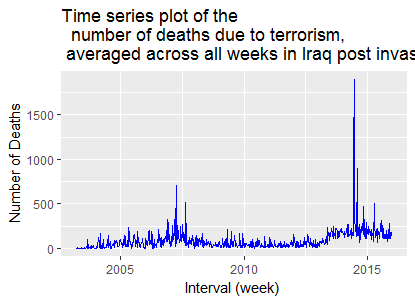
\includegraphics[width=10cm]{Peters_experiment_markdown_files/figure-latex/Rplot03_weekly_death_counts_iraq.png}
\caption{Time series plot interval(week) of deaths}
\label{fig:tseriesweek}
\centering
\end{figure}

Initial Application of the Twitter outbreak algorithm was applied to terrorist deaths in Iraq, over the all data in the GTD pertaining to Iraq, and to Post invasion upto the pullout and post-pullout as two distinct periods. Using the twitter breakout detection algorithm, the algorithm was applied using a minimum number of transitions between change points of four weeks (approximately month). This seemed to be a reasonable time period so as to survey counts and compare to a minimum of four weeks previously. The time series plot over-layed with the detected outbreaks is shown in figure~\ref{fig:tseriesweektwitter outbreak} 

\begin{figure}[t]
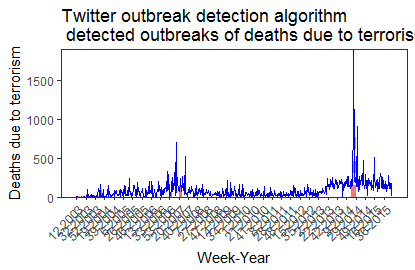
\includegraphics[width=10cm]{Peters_experiment_markdown_files/figure-latex/Rplot02_Twitter_outbreak_detection_algo.png}
\caption{Time series plot interval(week) of deaths and application of twitter outbreak detection algorithm. The detected outbreaks are shown indicated as vertical red lines}
\label{fig:tseriesweektwitter outbreak}
\centering
\end{figure}

The breakout detection algorithm showed a number of  breakout of incidents upto the surge, break outs are seen approximately 6 months after the invasion, these breakouts become frequent after this initial period with a break out occurring more frequently upto the surge and after and post-pullout at the time of the major ISIS offensive. A table of identified breakouts in Iraq is shown below in table~\ref{tab:labelsiraq}. 
Outbreaks are detected almost immediately after the invasion, however they seem to be extremely intermittent. Outbreaks are again detected at the end of 2003 and at the start of 2004. Outbreaks again are seen at the start 2007, which would correlate with the surge. An outbreak again is detected midway through 2007 which would correlate with the period of the US troop surge in Iraq. It is interesting to note that no outbreak (corresponding to mean or gradual shift downward trend in violence) is detected in the period post surge. 2012 sees a an outbreak detected at the end of the year which would correspond to the initial rise of ISIS.
 
% latex table generated in R 3.3.2 by xtable 1.8-2 package
% Sat Feb 25 19:58:45 2017
\begin{table}[ht]
\centering
\begin{tabular}{rrrrrl}
  \hline
 & year & week & sum\_kill & weekstrdate & wkyr \\ 
  \hline
 & 2003.00 & 15.00 & 2.00 & 1050274800.00 & 15-2003 \\ 
 & 2003.00 & 31.00 & 0.00 & 1059951600.00 & 31-2003 \\ 
 & 2003.00 & 35.00 & 100.00 & 1062370800.00 & 35-2003 \\ 
 & 2003.00 & 42.00 & 0.00 & 1066604400.00 & 42-2003 \\ 
 & 2003.00 & 47.00 & 26.00 & 1069632000.00 & 47-2003 \\ 
 & 2004.00 & 4.00 & 10.00 & 1075075200.00 & 4-2004 \\ 
 & 2004.00 & 9.00 & 168.00 & 1078099200.00 & 9-2004 \\ 
 & 2007.00 & 2.00 & 28.00 & 1168819200.00 & 2-2007 \\ 
 & 2007.00 & 23.00 & 242.00 & 1181516400.00 & 23-2007 \\ 
 & 2012.00 & 52.00 & 6.00 & 1356307200.00 & 52-2012 \\ 
 & 2014.00 & 22.00 & 147.00 & 1401663600.00 & 22-2014 \\ 
 & 2014.00 & 26.00 & 195.00 & 1404082800.00 & 26-2014 \\ 
   \hline
\end{tabular}
\caption{Identified breakouts of deaths due to terrorism in Iraq post invasion}
\label{tab:labelsiraq} 
\end{table}

The same dataset was examined using the SURUS RAD algorithm. The detected outliers are shown in Figure~\ref{fig:tseriessurusrad}. The low rank signal is represented in blue and is a pretty decent approximation of the underlying trend bar the outliers, which are represented as red circles with the size representing the magnitude of the outlier. The green line represents the underlying noise in the signal. The table detailing the outliers are in table~\ref{tab:RADTABLE}. The magnitude of the outlier is denoted in the S\_ Transform column. A high frequency of outliers are detected throughout 2006, this is correlated with the heightening of a bitter sectarian war in Iraq and the coming to the fore of AL-Qa'ida in iraq as the pre-eminent Sunni armed opposition to the US led invasion \citep{fearon2007iraq}. The US troop surge \citep{ricks2009gamble} is also correlated with a large number of outliers in deaths due to terrorism. There is also a high frequency of at the start of 2013 this would correlate with the change point detected using the twitter outbreak detection algorithm in table~\ref{tab:labelsiraq}. This correlates with the real world events of rise of ISIS in Iraq and Syria [needs more detailed citation see black flag book].


\begin{figure}[t]
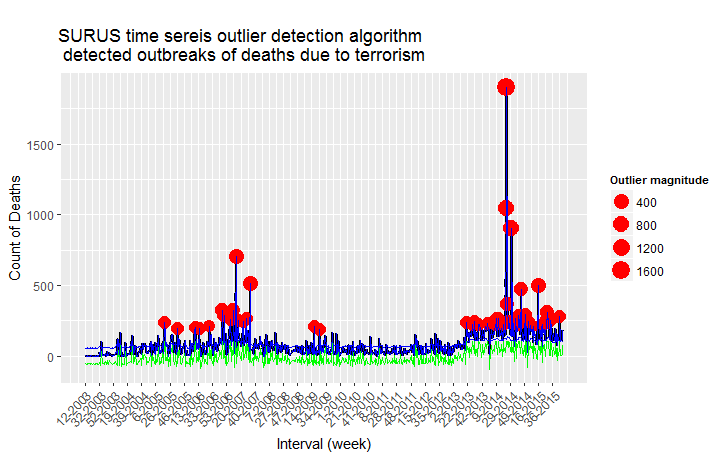
\includegraphics[width=10cm]{Peters_experiment_markdown_files/figure-latex/Surus_Rad_iraq.png}
\caption{Time series plot interval(week) of deaths and application of SURUS RAD algorithm.}
\label{fig:tseriessurusrad}
\centering
\end{figure}

% latex table generated in R 3.3.2 by xtable 1.8-2 package
% Sun Feb 26 00:33:27 2017
\begin{table}[ht]
\centering
\begin{tabular}{rrrrrl}
  \hline
 & X\_transform & L\_transform & S\_transform & E\_transform & wkyr \\ 
  \hline
 & 240.00 & 101.21 & 37.59 & 101.20 & 18-2005 \\ 
 & 194.00 & 84.37 & 8.43 & 101.20 & 37-2005 \\ 
 & 203.00 & 90.13 & 11.67 & 101.20 & 9-2006 \\ 
 & 195.00 & 88.31 & 5.49 & 101.20 & 14-2006 \\ 
 & 207.00 & 102.28 & 3.52 & 101.20 & 29-2006 \\ 
 & 325.00 & 94.50 & 129.30 & 101.20 & 47-2006 \\ 
 & 289.00 & 105.05 & 82.75 & 101.20 & 49-2006 \\ 
 & 259.00 & 110.48 & 47.32 & 101.20 & 5-2007 \\ 
 & 323.00 & 100.38 & 121.42 & 101.20 & 10-2007 \\ 
 & 707.00 & 109.40 & 496.40 & 101.20 & 13-2007 \\ 
 & 255.00 & 109.82 & 43.98 & 101.20 & 16-2007 \\ 
 & 242.00 & 100.38 & 40.42 & 101.20 & 23-2007 \\ 
 & 268.00 & 97.75 & 69.05 & 101.20 & 27-2007 \\ 
 & 517.00 & 82.64 & 333.16 & 101.20 & 33-2007 \\ 
 & 212.00 & 82.62 & 28.18 & 101.20 & 17-2009 \\ 
 & 187.00 & 78.79 & 7.01 & 101.20 & 25-2009 \\ 
 & 239.00 & 96.05 & 41.75 & 101.20 & 20-2013 \\ 
 & 227.00 & 118.54 & 7.26 & 101.20 & 28-2013 \\ 
 & 248.00 & 113.07 & 33.73 & 101.20 & 32-2013 \\ 
 & 225.00 & 109.61 & 14.19 & 101.20 & 37-2013 \\ 
 & 228.00 & 110.01 & 16.79 & 101.20 & 50-2013 \\ 
 & 223.00 & 114.77 & 7.03 & 101.20 & 8-2014 \\ 
 & 264.00 & 122.33 & 40.47 & 101.20 & 10-2014 \\ 
 & 264.00 & 119.12 & 43.68 & 101.20 & 12-2014 \\ 
 & 227.00 & 114.71 & 11.09 & 101.20 & 19-2014 \\ 
 & 1045.00 & 123.45 & 820.35 & 101.20 & 23-2014 \\ 
 & 1898.00 & 120.26 & 1676.54 & 101.20 & 24-2014 \\ 
 & 363.00 & 136.28 & 125.52 & 101.20 & 25-2014 \\ 
 & 248.00 & 134.34 & 12.46 & 101.20 & 27-2014 \\ 
 & 903.00 & 112.38 & 689.42 & 101.20 & 31-2014 \\ 
 & 231.00 & 110.92 & 18.88 & 101.20 & 34-2014 \\ 
 & 266.00 & 108.71 & 56.09 & 101.20 & 36-2014 \\ 
 & 226.00 & 114.03 & 10.77 & 101.20 & 40-2014 \\ 
 & 284.00 & 131.53 & 51.27 & 101.20 & 41-2014 \\ 
 & 247.00 & 129.93 & 15.87 & 101.20 & 42-2014 \\ 
 & 472.00 & 126.06 & 244.74 & 101.20 & 44-2014 \\ 
 & 291.00 & 118.22 & 71.58 & 101.20 & 50-2014 \\ 
 & 243.00 & 105.15 & 36.65 & 101.20 & 2-2015 \\ 
 & 212.00 & 108.51 & 2.29 & 101.20 & 9-2015 \\ 
 & 503.00 & 99.53 & 302.27 & 101.20 & 15-2015 \\ 
 & 225.00 & 113.87 & 9.93 & 101.20 & 22-2015 \\ 
 & 256.00 & 107.25 & 47.55 & 101.20 & 27-2015 \\ 
 & 262.00 & 130.61 & 30.19 & 101.20 & 28-2015 \\ 
 & 309.00 & 129.04 & 78.76 & 101.20 & 29-2015 \\ 
 & 237.00 & 128.88 & 6.92 & 101.20 & 30-2015 \\ 
 & 252.00 & 111.99 & 38.81 & 101.20 & 33-2015 \\ 
 & 282.00 & 107.73 & 73.07 & 101.20 & 46-2015 \\ 
   \hline
\end{tabular}
\caption{Output of RAD detection algorithm}
\label{tab:RADTABLE}
\end{table}

\subsection{The use of syndromic surveillance methods (EARSC3 and surveillance methods) to analyse Iraqi Death counts due to terrorism} 

As stated previously both EARSC3 and Farrington's syndromic surveillance algorithm were applied to Iraq data. In both cases, the only data preparation required was minimal, with the dataframe of counts by week requiring casting as an sts (surveillance time series) object before applying the surveillance algorithm. The output though as with the previous plots (of the SURUS outlier detection algorithm and the twitter outbreak detection algorithm) were enhanced by plotting them with ggplot. For the EARSC3 algorithm, a baseline of 18 weeks (4 months roughly) was chosen (which roughly responds to a  quadrimestral review period, this was alos used for the Farrington algorithm). The detected syndromic surveillance outbreaks are shown in figure~\ref{fig:tseriesEARSC3RAD}. A table showing the alarms raised by algorithm are shown in \ref{tab:tseriesEARSC3RADtable}. The plot shows the alarms raised (indicating an outbreak) as red circles, the count of deaths is shown as the black line and the blue line represents the threshold. 


\begin{figure}[t]
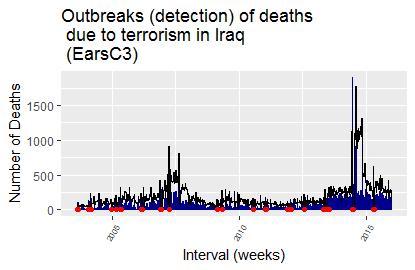
\includegraphics[width=10cm]{Peters_experiment_markdown_files/figure-latex/Rplot02_EarsC3.png}
\caption{Time series plot interval(week) of deaths and application of EARSC3 algorithm}
\label{fig:tseriesEARSC3RAD}
\centering
\end{figure}

% latex table generated in R 3.3.2 by xtable 1.8-2 package
% Sun Feb 26 21:52:18 2017
\begin{table}[ht]
 \begin{adjustwidth}{-2cm}{}
\begin{tabular}{llllllllll}
  \hline
 & observed & epoch & state & alarm & upperbound & population & freq & epochInPeriod & time \\ 
  \hline
 & 100.00 & 1062370778.00 & FALSE & TRUE & 81.26 & 1.00 & 52.00 & 0.90 & 2003-08-25 \\ 
 & 1.00 & 1062975578.00 & FALSE & TRUE & 0.00 & 1.00 & 52.00 & 0.67 & 2003-09-01 \\ 
 & 6.00 & 1063580378.00 & FALSE & TRUE & 0.00 & 1.00 & 52.00 & 0.44 & 2003-09-08 \\ 
 & 118.00 & 1076284778.00 & FALSE & TRUE & 34.16 & 1.00 & 52.00 & 0.83 & 2004-02-02 \\ 
 & 19.00 & 1076889578.00 & FALSE & TRUE & 0.00 & 1.00 & 52.00 & 0.60 & 2004-02-09 \\ 
 & 10.00 & 1077494378.00 & FALSE & TRUE & 0.00 & 1.00 & 52.00 & 0.37 & 2004-02-16 \\ 
 & 28.00 & 1079308778.00 & FALSE & TRUE & 0.00 & 1.00 & 52.00 & 0.67 & 2004-03-08 \\ 
 & 7.00 &  & FALSE & TRUE & 5.99 & 1.00 & 52.00 &  & 2004-12-27 \\ 
 & 19.00 & 1110758378.00 & FALSE & TRUE & 0.00 & 1.00 & 52.00 & 0.67 & 2005-03-07 \\ 
 & 158.00 & 1115593178.00 & FALSE & TRUE & 102.79 & 1.00 & 52.00 & 0.60 & 2005-05-02 \\ 
 & 73.00 & 1116197978.00 & FALSE & TRUE & 0.00 & 1.00 & 52.00 & 0.37 & 2005-05-09 \\ 
 & 203.00 & 1140998378.00 & FALSE & TRUE & 152.51 & 1.00 & 52.00 & 0.13 & 2006-02-20 \\ 
 & 46.00 & 1141603178.00 & FALSE & TRUE & 0.00 & 1.00 & 52.00 & 0.90 & 2006-02-27 \\ 
 & 83.00 & 1142207978.00 & FALSE & TRUE & 16.50 & 1.00 & 52.00 & 0.67 & 2006-03-06 \\ 
 & 80.00 & 1164585578.00 & FALSE & TRUE & 0.00 & 1.00 & 52.00 & 0.13 & 2006-11-20 \\ 
 & 289.00 & 1165190378.00 & FALSE & TRUE & 196.96 & 1.00 & 52.00 & 0.90 & 2006-11-27 \\ 
 & 137.00 & 1165795178.00 & FALSE & TRUE & 55.46 & 1.00 & 52.00 & 0.67 & 2006-12-04 \\ 
 & 50.00 & 1166399978.00 & FALSE & TRUE & 0.00 & 1.00 & 52.00 & 0.44 & 2006-12-11 \\ 
 & 60.00 & 1176073178.00 & FALSE & TRUE & 0.00 & 1.00 & 52.00 & 0.52 & 2007-04-02 \\ 
 & 137.00 & 1176677978.00 & FALSE & TRUE & 0.00 & 1.00 & 52.00 & 0.29 & 2007-04-09 \\ 
 & 5.00 & 1235347178.00 & FALSE & TRUE & 0.00 & 1.00 & 52.00 & 0.13 & 2009-02-16 \\ 
 & 21.00 & 1235951978.00 & FALSE & TRUE & 8.75 & 1.00 & 52.00 & 0.90 & 2009-02-23 \\ 
 & 19.00 & 1241391578.00 & FALSE & TRUE & 0.00 & 1.00 & 52.00 & 0.60 & 2009-04-27 \\ 
 & 10.00 & 1241996378.00 & FALSE & TRUE & 0.00 & 1.00 & 52.00 & 0.37 & 2009-05-04 \\ 
 & 29.00 & 1280703578.00 & FALSE & TRUE & 16.91 & 1.00 & 52.00 & 0.60 & 2010-07-26 \\ 
 & 94.00 & 1295827178.00 & FALSE & TRUE & 90.38 & 1.00 & 52.00 & 0.06 & 2011-01-17 \\ 
 & 17.00 & 1296431978.00 & FALSE & TRUE & 0.00 & 1.00 & 52.00 & 0.83 & 2011-01-24 \\ 
 & 67.00 & 1323043178.00 & FALSE & TRUE & 62.86 & 1.00 & 52.00 & 0.67 & 2011-11-28 \\ 
 & 24.00 & 1323647978.00 & FALSE & TRUE & 0.08 & 1.00 & 52.00 & 0.44 & 2011-12-05 \\ 
 & 106.00 & 1326067178.00 & FALSE & TRUE & 51.38 & 1.00 & 52.00 & 0.52 & 2012-01-02 \\ 
 & 61.00 & 1326671978.00 & FALSE & TRUE & 0.00 & 1.00 & 52.00 & 0.29 & 2012-01-09 \\ 
 & 109.00 & 1327276778.00 & FALSE & TRUE & 91.72 & 1.00 & 52.00 & 0.06 & 2012-01-16 \\ 
 & 92.00 & 1343602778.00 & FALSE & TRUE & 70.18 & 1.00 & 52.00 & 0.60 & 2012-07-23 \\ 
 & 63.00 & 1344207578.00 & FALSE & TRUE & 21.38 & 1.00 & 52.00 & 0.37 & 2012-07-30 \\ 
 & 86.00 & 1367794778.00 & FALSE & TRUE & 84.48 & 1.00 & 52.00 & 0.37 & 2013-04-29 \\ 
 & 40.00 & 1368399578.00 & FALSE & TRUE & 35.73 & 1.00 & 52.00 & 0.13 & 2013-05-06 \\ 
 & 140.00 & 1369609178.00 & FALSE & TRUE & 45.56 & 1.00 & 52.00 & 0.67 & 2013-05-20 \\ 
 & 151.00 & 1370213978.00 & FALSE & TRUE & 6.22 & 1.00 & 52.00 & 0.44 & 2013-05-27 \\ 
 & 157.00 & 1370818778.00 & FALSE & TRUE & 59.79 & 1.00 & 52.00 & 0.21 & 2013-06-03 \\ 
 & 94.00 & 1371423578.00 & FALSE & TRUE & 48.96 & 1.00 & 52.00 & 0.98 & 2013-06-10 \\ 
 & 188.00 & 1375052378.00 & FALSE & TRUE & 185.63 & 1.00 & 52.00 & 0.60 & 2013-07-22 \\ 
 & 1898.00 & 1402873178.00 & FALSE & TRUE & 1161.16 & 1.00 & 52.00 & 0.98 & 2014-06-09 \\ 
 & 363.00 & 1403477978.00 & FALSE & TRUE & 0.00 & 1.00 & 52.00 & 0.75 & 2014-06-16 \\ 
 & 195.00 & 1404082778.00 & FALSE & TRUE & 0.00 & 1.00 & 52.00 & 0.52 & 2014-06-23 \\ 
 & 248.00 & 1404687578.00 & FALSE & TRUE & 0.00 & 1.00 & 52.00 & 0.29 & 2014-06-30 \\ 
 & 201.00 & 1429484378.00 & FALSE & TRUE & 41.23 & 1.00 & 52.00 & 0.83 & 2015-04-13 \\ 
 & 185.00 & 1430089178.00 & FALSE & TRUE & 16.89 & 1.00 & 52.00 & 0.60 & 2015-04-20 \\ 
   \hline
\end{tabular}
\caption{A table of alarms raised by the EARSC3 algorithm}
\end{adjustwidth}
\label{tab:tseriesEARSC3RADtable}
\end{table}


